\documentclass{amsart}

\usepackage[english]{babel}
\usepackage[utf8]{inputenc}
\usepackage{graphicx}
\usepackage{mathtools}
\usepackage{amsthm}
\usepackage{thmtools,thm-restate}
\usepackage{amsfonts}
\usepackage{hyperref}
\usepackage[singlelinecheck=false]{caption}
\usepackage[backend=biber,url=true,doi=true,eprint=false,style=alphabetic]{biblatex}
\usepackage{enumitem}
\usepackage[justification=centering]{caption}
\usepackage{indentfirst}
\usepackage{algorithm}
\usepackage{algpseudocode}
\usepackage{listings}
\usepackage[x11names, rgb]{xcolor}
\usepackage{tikz}
\usepackage{hyperref}
\usepackage{subcaption}
\usepackage{booktabs}
\usepackage{linegoal}
\usetikzlibrary{snakes,arrows,shapes}

\addbibresource{references.bib}

\makeatletter
\def\subsection{\@startsection{subsection}{3}%
  \z@{.5\linespacing\@plus.7\linespacing}{.1\linespacing}%
  {\normalfont}}
\makeatother

\makeatletter
\patchcmd{\@setauthors}{\MakeUppercase}{}{}{}
\makeatother

\DeclareMathOperator*{\argmin}{arg\,min}
\DeclareMathOperator*{\argmax}{arg\,max}
\DeclareMathOperator*{\Val}{\text{Val}}
\DeclareMathOperator*{\Ch}{\text{Ch}}
\DeclareMathOperator*{\Pa}{\text{Pa}}
\DeclareMathOperator*{\Sc}{\text{Sc}}
\newcommand{\ov}{\overline}

\newcommand\defeq{\mathrel{\overset{\makebox[0pt]{\mbox{\normalfont\tiny\sffamily def}}}{=}}}

\newcommand{\algorithmautorefname}{Algorithm}
\algrenewcommand\algorithmicrequire{\textbf{Input}}
\algrenewcommand\algorithmicensure{\textbf{Output}}
\algnewcommand{\LineComment}[1]{\State\,\(\triangleright\) #1}

\captionsetup[table]{labelsep=space}

\theoremstyle{plain}

\newcounter{dummy-def}\numberwithin{dummy-def}{section}
\newtheorem{definition}[dummy-def]{Definition}
\newcounter{dummy-thm}\numberwithin{dummy-thm}{section}
\newtheorem{theorem}[dummy-thm]{Theorem}
\newcounter{dummy-prop}\numberwithin{dummy-prop}{section}
\newtheorem{proposition}[dummy-prop]{Proposition}
\newcounter{dummy-corollary}\numberwithin{dummy-corollary}{section}
\newtheorem{corollary}[dummy-corollary]{Corollary}
\newcounter{dummy-lemma}\numberwithin{dummy-lemma}{section}
\newtheorem{lemma}[dummy-lemma]{Lemma}
\newcounter{dummy-ex}\numberwithin{dummy-ex}{section}
\newtheorem{exercise}[dummy-ex]{Exercise}
\newcounter{dummy-eg}\numberwithin{dummy-eg}{section}
\newtheorem{example}[dummy-eg]{Example}

\numberwithin{equation}{section}

\newcommand{\set}[1]{\mathbf{#1}}
\newcommand{\pr}{\mathbb{P}}
\renewcommand{\implies}{\Rightarrow}

\newcommand{\bigo}{\mathcal{O}}

\setlength{\parskip}{1em}

\lstset{frameround=fttt,
	numbers=left,
	breaklines=true,
	keywordstyle=\bfseries,
	basicstyle=\ttfamily,
}

\newcommand{\code}[1]{\lstinline[mathescape=true]{#1}}
\newcommand{\mcode}[1]{\lstinline[mathescape]!#1!}


\title{%
  \noindent\rule{13cm}{1.0pt}\\
  \vspace{0.2cm}
  Analysis on an Implementation of the Gens-Domingos Sum-Product Network Structural Learning
  Schema
  \noindent\rule{13cm}{0.8pt}
}
\xdef\shorttitle{Analysis on the GD Schema}
\author[]{\normalsize\textbf{Renato Lui Geh}\\\small Computer Science\\Institute of Mathematics
  and Statistics\\University of São Paulo\\\texttt{renatolg@ime.usp.br}}

\begin{document}

\begin{abstract}
  Sum-Product Networks (SPNs) are a class of deep probabilistic graphical models. Inference in them
  is linear in the number of edges of the graph. Furthermore, exact inference is achieved, in a
  valid SPN, by running through its edges twice at most, making exact inference linear. The
  Gens-Domingos SPN Schema is an algorithm for structural learning on such models. In this paper we
  present an implementation of such schema, analyzing its complexity, discoursing implementational
  and theoretical details, and finally presenting results and experiments achieved with this
  implementation.

  \smallskip
  \smallskip
  \smallskip
  \textbf{Keywords}
  \smallskip
  \texttt{cluster analysis; data mining; probabilistic graphical models; tractable models; machine
  learning; deep learning}
  \vspace*{-3.5em}
\end{abstract}

\maketitle

\section{Introduction}

A Sum-Product Network (SPN) is a probabilistic graphical model that represents a tractable
distribution of probability. If an SPN is valid, then we can perform exact inference in time linear
to the graph's edges. Its syntax is different to other conventional models (read bayesian and
markov networks) in the sense that its graph does not explicitly model events and
(in)\,dependencies between variables. That is, whilst variables in a bayesian network are
represented as nodes in the graph, with each edge connecting two nodes asserting a dependency
relationship between the connected variables, a node in an SPN may not necessarily represent a
variable or event, neither an edge connecting two nodes represent dependence. In this sense, SPNs
can be seen as a type of probabilistic Artificial Neural Network (ANN). However, whilst neural
networks represent a function, SPNs model a tractable probability distribution. Furthermore, SPNs
are distinct from standard neural networks seeing that, whereas ANNs have only one type of neuron
with an activation function mapping to values in $[0,1]$, SPNs have two kinds of neurons, which we
will see in the next sections. Still, SPNs retain certain important characteristics from ANNs as we
will discuss later, with mainly its deep structure properties~\cite{shallow-vs-deep} as the most
interesting feature.

The Gens-Domingos Schema~\cite{gens-domingos}, or \code{LearnGD} as we will reference it throughout
this paper, is an SPN structural learning algorithm proposed by Robert Gens and Pedro Domingos.
Gens and Domingos call it a schema because it only provides a template of what the algorithm should
be like. We will discuss \code{LearnGD} in details in the next section. This paper documents a
particular implementation of the GD schema. Other implementations may have different results.

In this document, we show how we implemented the \code{LearnGD} algorithm. We analyze the
complexity of each algorithm component in detail, later referring to such analyses when drawing
conclusions on the overall complexity of the algorithm. As we have mentioned before, since the
\code{LearnGD} schema heavily depends on implementation, the complexity we achieve in this
particular case may differ from other implementations. After each analysis, we then look at the
algorithm as a whole, drawing conclusions on time and memory usage, as well as implementation
details that could potentially decrease the algorithm runtime. We also comment on how to implement
better concurrency then how it is currently coded in our implementation. We then show some results
on experiments made on image classification and image completion.

\section{Sum-Product Networks}

In this section we will define SPNs differently from other articles~\cite{gens-domingos,
poon-domingos, clustering} as the original more convoluted definition is of little use for the
\code{LearnGD} algorithm. Our definition is almost identical to the original \code{LearnGD} article
\cite{gens-domingos}, with the exception that we assume that an SPN is already normalized. This
fact changes nothing, since Peharz \textit{et al} recently proved that normalized SPNs have as much
representability power as unnormalized SPNs~\cite{theoretical-spn}. Before we enunciate the formal
definition of an SPN, we will give an informal, vague definition of an SPN in order to explain what
completeness, consistency, validity and decomposability --- which are an important set of
definitions --- of an SPN mean.

A sum-product network represents a tractable probability distribution through a DAG\@. Such digraph
must always be weakly connected. A node can either be a leaf, a sum, or a product node. The scope
of a node is the set of all variables present in all its descendants. Leaf nodes are tractable
probability distributions and their scope is the scope of its distribution, sum nodes represent the
summing out of the variables in its scope and product nodes act as feature hierarchy. An edge that
has its origin from a sum node has a non-negative weight. We refer to a sub-SPN $S$ rooted at node
$i$ as $S(i)$, while the SPN rooted at its root is denoted as $S(\cdot)$ or simply $S$. The scope
of a node will be denoted as $\Sc(i)$, where $i$ is a node. The set of children of a node will be
denoted as $\Ch(i)$. Similarly, $\Pa(i)$ is the set of parents of node $i$.

\begin{definition}[Normalized]~\\
  Let $S$ be an SPN and $\Sigma(S)$ be the set of all sum nodes of $S$. $S$ is normalized iff, for
  all $\sigma \in \Sigma(S)$, $\sum_{c\in Ch(\sigma)} w_{\sigma c} = 1$ and $0 \leq w_{\sigma c}
  \leq 1$, where $w_{\sigma c}$ is the weight from edge $\sigma \to c$.
\end{definition}

\begin{definition}[Completeness]~\\
  Let $S$ be an SPN and $\Sigma(S)$ be the set of all sum nodes of $S$. $S$ is complete iff, for
  all $\sigma \in \Sigma(S)$, $\Sc(i)=\Sc(j), i\neq j; \forall i,j\in \Ch(\sigma)$.
\end{definition}

\begin{definition}[Consistency]~\\
  Let $S$ be an SPN, $\Pi(S)$ be the set of all product nodes of $S$ and $X$ a variable in
  $\Sc(S)$. $S$ is consistent iff $X$ takes the same value for all elements in $\Pi(S)$ that
  contain $X$.
\end{definition}

\begin{definition}[Validity]~\\
  An SPN $S$ is valid iff it always computes the correct probability of evidence $S$ represents.
\end{definition}

\begin{theorem}\label{thm:validity}
  An SPN $S$ is valid if it is both complete and consistent.
\end{theorem}

Validity guarantees that the SPN will compute not only the correct probability of evidence, but
also in time linear to its graph's edges. Therefore, it is preferable to learn valid SPNs. Notice
that~\autoref{thm:validity} is not restricted by completeness and consistency. In fact, incomplete
and/or inconsistent SPNs can compute the probability of evidence correctly, but consistency and
completeness guarantee that all sub-SPNs are also valid.

\begin{definition}[Decomposability]~\\
  Let $S$ be an SPN and $\Pi(S)$ be the set of all product nodes in $S$. $S$ is decomposable iff,
  for all $\pi \in \Pi(S)$, $\Sc(i)\cap \Sc(j)=\emptyset, i\neq j; \forall i,j\in \Ch(\pi)$.
\end{definition}

It is clear that decomposability implies consistency, therefore if an SPN is both complete and
decomposable, than it is also valid. We choose to work with decomposability because it is easier to
learn decomposable SPNs then it is to learn consistent ones. We do not lose representation power
because a complete and consistent SPN can be transformed into a complete and decomposable SPN in no
more than a polynomial number of edge and node additions~\cite{theoretical-spn}. We can now
formally define an SPN\@.

\begin{definition}[Sum-product network]~\\
  A sum-product network (SPN) is a weakly connected DAG that can be recursively defined as
  following.

  An SPN\@:
  \begin{enumerate}
    \item with a single node is a univariate tractable probability distribution (\textbf{leaf});
    \item is a normalized weighted sum of SPNs of same scope (\textbf{sum});
    \item is a product of SPNs with disjoint scopes (\textbf{product}).
  \end{enumerate}
  The value of an SPN is defined by its type. Let $\lambda$, $\sigma$ and $\pi$ be a leaf, sum and
  product respectively. The values of such SPNs are given by $\lambda(\mathbf{x})$,
  $\sigma(\mathbf{x})$ and $\pi(\mathbf{x})$, where $\mathbf{x}$ is a certain evidence
  instantiation.
  \begin{description}
    \item[Leaf] $\lambda(\mathbf{x})$ is the value of the probability distribution at point
      $\mathbf{x}$.
    \item[Product] $\pi(\mathbf{x}) = \prod_{c \in \Ch(\pi)} c(\mathbf{x})$.
    \item[Sum] $\sigma(\mathbf{x}) = \sum_{c \in \Ch(\sigma)} w_{\sigma c} c(\mathbf{x})$, with
      $\sum_{c \in \Ch(\sigma)} w_{\sigma c} = 1$ and $0 \leq w_{\sigma c} \leq 1$.
  \end{description}
\end{definition}

Note that this definition assumes an SPN to be complete, decomposable and normalized. Other
definitions in literature may differ from ours, but as we have mentioned before, for our
implementation, this definition is convenient for us. Another observation worthy of notice is the
value of $\lambda(\mathbf{x})$. Although here we consider $\mathbf{x}$ to be a multivariate
instantiation (i.e.\ a set of --- potentially multiple --- variable valuations), we had initially
defined a leaf to be a univariate distribution. Although it is possible to attribute leaves as
multivariate probability distributions~\cite{id-spn}, for our definition we have chosen to keep a
leaf's scope a unit set. Therefore, in the case of a leaf's value, $\mathbf{x}$ is a singleton
(univariate) variable instantiation.

\section{The \code{LearnGD} Schema}

The \code{LearnGD} schema was proposed by Robert Gens and Pedro Domingos on \textit{Learning the
Structure of Sum-Product Networks}~\cite{gens-domingos}. In this section we will outline the schema
in pseudo-code and analyze a few properties derived from the algorithm.

\begin{algorithm}[H]
  \caption{\code{LearnGD}}\label{alg:learngd}
  \begin{algorithmic}[1]
    \Require\,Set $\mathbf{D}$ of instances (data)
    \Require\,Set $\mathbf{V}$ of variables (scope)
    \Ensure\,An SPN representing a probability distribution given by $\mathbf{D}$ and $\mathbf{V}$
    \If{$|\set{V}|=1$} \Comment{univariate data sample}
      \State\,\textbf{return} univariate distribution estimated from $T[\set{V}]$ (data of
        $\set{V}$)
    \EndIf%
    \State\,Take $\set{V}$ and find mutually independent subsets $\set{V}_i$ of variables
    \If{possible to partition} \Comment{i.e.\ we have found independent subsets}
      \State\,\textbf{return} $\prod_i$ \mcode{LearnGD ($\set{D}$, $\set{V}_i$)}
    \Else\Comment{we cannot say there is independence}
      \State\,Take $\set{D}$ and find $\set{D}_j$ subsets of similar instances
      \If{possible to partition}
        \State\,\textbf{return} $\sum_i \frac{|\set{D}_j|}{|\set{D}|} \cdot$ \mcode{LearnGD
        ($\set{D}_j$, $\set{V}$)}
      \Else\Comment{i.e.\ data is one big cluster}
        \State\,\textbf{return} fully factorized distribution.
      \EndIf%
    \EndIf%
  \end{algorithmic}
\end{algorithm}

Let us now, for a moment, suppose that SPNs are not necessarily complete, decomposable and
normalized. We shall prove a few results derived from SPNs generated by~\autoref{alg:learngd}.

\begin{lemma}
  An SPN $S$ generated by \code{LearnGD} is complete, decomposable and normalized.
\end{lemma}
\begin{proof}
  Lines 4--6 show that the scope of each child in a product node of $S$ is a partition of the scope
  of their parent. Therefore, children have pairwise disjoint scopes on line 6, which proves
  decomposability for this part of the algorithm. In lines 8--10, since we are clustering similar
  instances, $\set{D}$ is being partitioned but we are not changing $\set{V}$ in any way. In fact,
  line 10 shows that we pass $\set{V}$ to all other children. That is, all children of sum nodes
  have the same scope as their parent, which proves completeness.  Let $\set{D}_1,\ldots,\set{D}_n$
  be the subsets of similar instances. By the definition of clustering, $\set{D}_1\cup\ldots\cup
  \set{D}_n=\set{D}$ and $\set{D}_i\cap \set{D}_j= \emptyset$, $i\neq j$, $1\leq i,j\leq n$. Thus
  it follows that $\sum_{i=1}^n \frac{|\set{D}_i|}{|\set{D}|}=1$ and thus line 10 always creates
  complete and normalized sum nodes. Line 12 is a special case where, if we have discovered that
  $\set{D}$ is one big data cluster, we shall create a product node $\pi$ in which all children of
  $\pi$ are leaves and \begin{equation*} \bigcup_{\lambda\in\Ch(\pi)} \Sc(\lambda) = \Sc(\pi).
  \end{equation*} In other words, we fully factorize our product node into leaves. In this case, it
  is obvious that this product node is decomposable.
\end{proof}

\code{LearnGD} can be divided into four parts:

\begin{enumerate}
  \item Is the data univariate? If it is, return a leaf.
  \item Are partitions of the data independent? If they are, return a product node whose children
    are the independent partitions.
  \item Are partitions of the data similar? If they are, return a sum node whose children are the
    partition clusters.
  \item In case all else fails, we have a fully factorized distribution.
\end{enumerate}

Going back to our definition of an SPN, we can now take a more intuitive approach and make the
following observations:

\begin{enumerate}
  \item A leaf is nothing but a local/partitioned/sample distribution of a probability distribution
    given by a single variable.
  \item A product node determines independence between variables.
  \item A sum node is a clustering of similar data values (i.e.\ instances that are ``alike'').
\end{enumerate}

This gives more semantic value to SPNs, whilst still retaining its expressivity. Following this
approach, one can easily notice that each ``layer'' corresponds to a recursive call in
\code{LearnGD}. In fact, each recursive call constructs a hidden layer that tries to partition the
SPN even further. This gives SPNs a deep architecture that resembles deep models in that the deeper
the model, the more representation power it has~\cite{shallow-vs-deep}.

Let us now observe the scope of each type of node. A leaf is the trivial case, since it has a
single variable in its scope by definition. Each layer above it can have either sum or product
nodes. Let us now look at decomposability, that is: if a variable $X$ appears in a child of a
product node $\pi$, then $X$ cannot appear in another child of $\pi$. This gives us the following
result:

\begin{lemma}\label{lemma-parents}
  Let $S$ be an SPN generated by \code{LearnGD}, and let $\Lambda(S)$ be the set of all leaves of
  $S$. Then, $\forall \lambda \in \Lambda(S)$, we have that, $\forall p \in \Pa(\lambda)$, $p$ is a
  product node.
\end{lemma}
\begin{proof}
  Our proof is by contradiction. Let us assume that $\exists p \in \Pa(\lambda)$ such that $p$ is
  a sum node and $\exists c^* \in \Ch(p)$ a leaf. From our assumption that $p$ is a sum node, we
  have that, since the SPN is complete, the scope of all children of $p$ are the same and are all
  equal to the scope of $p$. Now let $c \in \Ch(p)$. There must exist another child $c$ such that
  $c\neq c^*$ because of lines 5 and 9. From that we have $\Sc(c)=\Sc(c^*)$ because of
  completeness, and since $\Sc(c^*)$ is singular, then $c$ must also be leaf. But it is impossible
  to have leaves with same scope and same parent (line 1 from~\autoref{alg:learngd}). Therefore,
  $p$ is actually a product node.
\end{proof}

\begin{lemma}
  An SPN generated by \code{LearnGD} is a rooted tree.
\end{lemma}
\begin{proof}
  It suffices to show that for any vertex, its indegree is exactly one. We can prove that by saying
  that~\autoref{alg:learngd} never adds edges between two already existing vertices.
\end{proof}

\begin{definition}
  A sum-product network that is a rooted tree is called a sum-product tree (SPT).
\end{definition}

\begin{theorem}~\\
  Let $S$ be an SPT generated by \code{LearnGD}. Let $n=|\Sc(S)|$ and $m=|\set{D}|$, where
  $\set{D}$ is the data sent as parameter to \code{LearnGD}. Let $h$ be the height of $S$. Then
  \begin{equation*}
    1 \leq h \leq n + m - 1
  \end{equation*}
\end{theorem}
\begin{proof}
  Sketch of proof: every sum or product node creates one more hidden layer (increments SPT's height
  by one) and decrements either an instance (if sum node) or variable in node's scope (if product
  node) by one at least. Last (deepest) sum node must have at least two product nodes as children
  (following~\autoref{lemma-parents}), with each having one data instance each, therefore the
  number of layers created by sum nodes is at most $m-1$. Similarly for product nodes, if we want
  to maximize the number of layers, the deepest product node must have two leaves as children,
  bringing the total count of product nodes to $n-1$. Counting the last layer that is made out of
  leaves, we have $(n-1)+(m-1)+1=n+m-1$. Furthermore, the SPT has the form of alternated
  sum-product layers (a sum node will follow a product node and vice-versa). This guarantees that
  each sum node modifies the overall data enough that the independence test will judge an
  independent variable from all others. The base case $h=1$ is trivial: a size $1$ scope generates
  one leaf with distribution equal to data. The case $h=2$ is more interesting and occurs when all
  variables are dependent and belong to the same cluster.

  \textbf{TODO:} Reword this more formally and unambiguously. Also put this after the variable
  independence test and data clustering sections.
\end{proof}

From~\autoref{alg:learngd} we have learned that \code{LearnGD} can be structured into three parts.
The first is discovering variable independencies and judging whether we should partition $V$ and
create a new product node. The second is, if the first part has failed, we must find possible
clusters from the data we have. From these newly discovered clusters, we decide if we should create
another sum node and assign each of its children a partition of these clusters, or if these
clusters all form a single big all encompassing cluster. If this is the case, we create a new
product node whose children are the fully factorized form of the present data. Finally, the third
and last part is the base case. If the scope is of a single variable, we return the univariate
probability distribution given by the univariate data.

If we were to visualize our dataset as a table where rows are instances and columns are variables,
we could equate the algorithm as splitting, either horizontally or vertically, the dataset
according to our partitioning decisions. For instance, if we had decided that there was a certain
subset of variables that were independent of the rest of the variables, we would ``split'' our
dataset table vertically, with each subtable belonging to a variable subset. Similarly for cluster
partitioning, we would split our dataset table horizontally. \autoref{fig:splitting} illustrates
the procedures for variable splitting (\autoref{fig:split-v}) and instance splitting
(\autoref{fig:split-h}).

\begin{figure}[h]
  \centering
  \begin{subfigure}{0.49\linewidth}
    \centering
    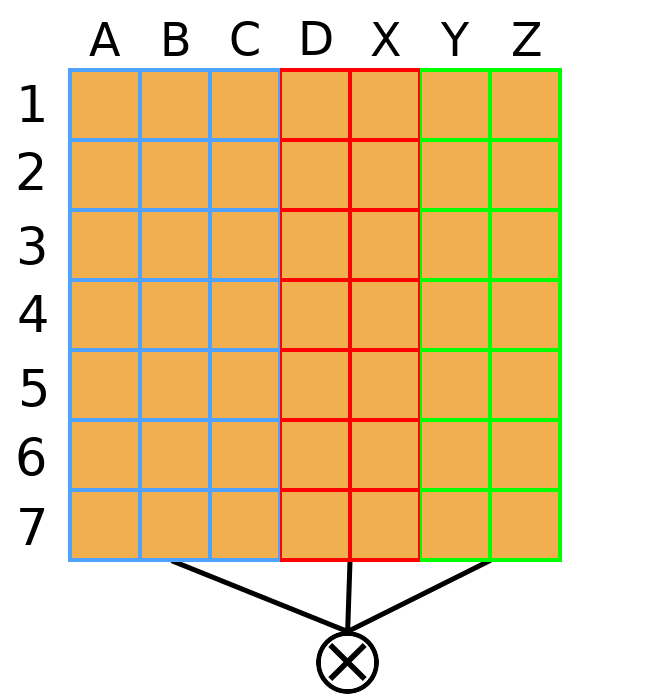
\includegraphics[scale=0.2]{imgs/split-v.png}
    \caption{~}\label{fig:split-v}
  \end{subfigure}
  \begin{subfigure}{0.49\linewidth}
    \centering
    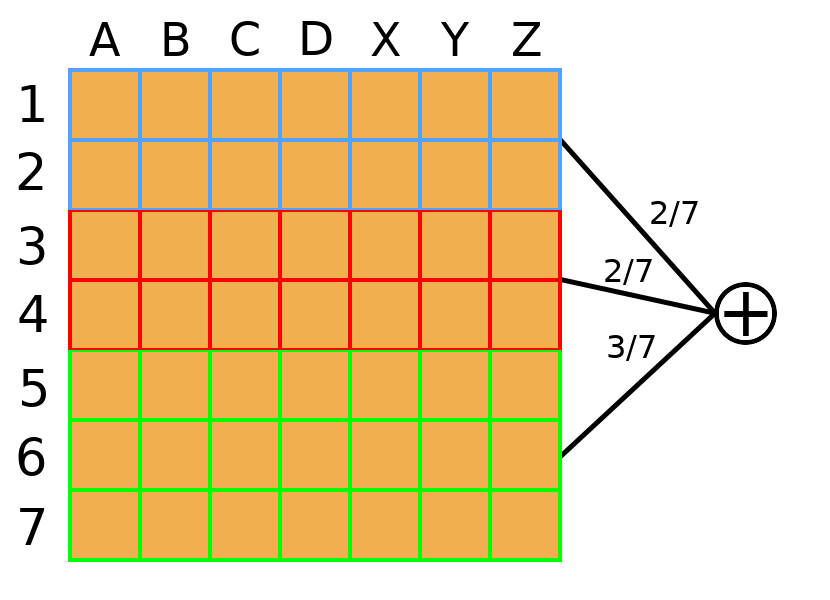
\includegraphics[scale=0.2]{imgs/split-h.png}
    \caption{~}\label{fig:split-h}
  \end{subfigure}
  \captionsetup{singlelinecheck=false,justification=justified,margin=0cm}
  \caption{These two images represent a dataset in table form. Rows are instances and columns are
  variables.\autoref{fig:split-v} shows variable splitting. In this example, we have observed that
  the subsets $\set{V}_1=\{A,B,C\}$, $\set{V}_2=\{D,X\}$ and $\set{V}_3=\{Y,Z\}$ are independent of
  each other. That is, for every pair $(P,Q), P\in \set{V}_i, Q\in \set{V}_j, i\neq j$, $P$ is
  independent of variable $Q$.  Given these partitions, we create a new product node whose children
  are the recursive calls to \code{LearnGD}. Note that their new scopes are now $V_i$, and their
  data instance covers only their new scope. In this example, the new partitions form subtables
  whose columns are adjacent to each other (e.g.\ $A$, $B$ and $C$ are adjacent). However, we could
  find an independent subset that did not necessarily obey a graphical rule, that is, we could have
  found that $A$ and $Y$ belong to the same partition. In this case, we would have considered $A$
  and $Y$ as a new subset, regardless of their graphical positions. For~\autoref{fig:split-h}, we
  apply a similar concept.  In this case we are clustering similar instances. Note that instance
  partitioning does not alter their scope. Each instance subset $\set{D}_1=\{1,2\}$,
  $\set{D}_2=\{3,4\}$ and $\set{D}_3=\{5,6,7\}$ equates to a discovered cluster. A new sum node is
  then created, with weights corresponding to the ratio of rows in each subtable. The subtables are
  then added as children of the sum node and then recursed. Just like with variable splitting,
  these partitions do not necessarily obey a graphical rule. We could have non-adjacent rows as a
single partition.}\label{fig:splitting} \end{figure}

Now that we have the general idea of the algorithm, we shall describe and analyze how to do both
variable and instance splitting. We will reserve a section to each of these topics. Once we have
covered them both, we shall once again take a broader look at the \code{LearnGD} schema and work on
some other results that depend on the two next sections.

\section{Variable Independence}

The core of variable splitting is finding independence between variables. What we wish to find is
partitions of the current SPN scope such that every element in a partition is independent of all
other elements in other partitions. In this section we shall explain the general idea, describe and
analyze the method used in our implementation and lastly discuss certain problems encountered
during experiments and implementation.

The description of our problem is: given a dataset with a set of variables $\mathbf{V}$, we wish to
find a set $\set{P}=\{\set{P}_1,\set{P}_2,\ldots,\set{P}_n\}$, where $\set{P}_i\cap
\set{P}_j=\emptyset, i\neq j$ and $\set{P}_1\cup \ldots\cup \set{P}_n=\mathbf{V}$ and $\set{P}_i$
is a subset of variables. That is, a set of partitions of $\mathbf{V}$. Additionally, for every
$\set{P}_i$ and $\set{P}_j$, $i\neq j$, $\forall u\in \set{P}_i, v\in \set{P}_j$, $u\perp v$ ($u$
is independent of $v$), where $\perp$ is the independence operator.

Suppose we have an independence oracle $\Omega$ that tells us if $X\perp Y$ and does so in constant
time. A naïve solution to this problem is, for every pair $X,Y \in \mathbf{V}$, ask $\Omega$ if
$X\perp Y$. We then memorize which ones are dependent and which are independent. For such
memoization, we can use an undirected graph.

\begin{definition}[Independence Graph]~\\
  Let $G=(\set{V},\set{E})$ be an undirected graph with vertex set $\set{V}$ and edge set
  $\set{E}$. Let $i$ and $j$ be vertices in $\set{V}$. There exists an edge $e_{ij}$ iff
  $i\not\perp j$.
\end{definition}

This reduces our problem to one of finding connected subgraphs. Since there exists an edge if and
only if the two connected variables are dependent, to find a partition $\set{P}_i$, it suffices to
find a connected subgraph in which all of its vertices have no path to another subgraph (there is
no dependence path between variables).

\begin{proposition}
  If $H=(\set{V}',\set{E'})$ is a connected subgraph in Independence Graph $G=(\set{V},\set{E})$
  then $\set{V}'\in\set{P}$.
\end{proposition}
\begin{proof}
  Since there cannot be two same variables in our graph, it suffices to show that, $\forall u'\in
  \set{V}', u\in \set{V}\setminus\set{V}'$: $u'\perp u$. Let us assume that $\set{V}'\not\in
  \set{P}$. That is, there exists an element in $\set{V}'$ that is dependent of an element in
  $\set{V}\setminus\set{V}'$. That means there exists a vertex $v'\in\set{V}'$ and another vertex
  $v\in\set{V}\setminus\set{V}'$ such that an edge $e_{v'v}$ connects both of them. But $u\in
  \set{V}\setminus\set{V}'$ and $\set{V}'$ is the vertex set of a connected subgraph, which means
  such an edge cannot exist, as there is no path from a vertex of $H$ to a vertex in $\set{V}
  \setminus\set{V}'$. Therefore our assumption that $\set{V}'\not\in\set{P}$ is false.
\end{proof}

Sketching our naïve solution, we have:

\begin{algorithm}[H]
  \caption{\code{IndepGraph}}\label{alg:indepgraph}
  \begin{algorithmic}[1]
    \Require\,Set $\mathbf{D}$ of instances (data)
    \Require\,Set $\mathbf{V}$ of variables (scope)
    \Ensure\,A set $\mathbf{P}$ of independent partitions of variables
    \State\,Let $\Omega$ be an independence oracle that returns true if independent and false if
      dependent
    \State\,Let $G=(\set{V},\set{E}=\emptyset)$ be an empty independence graph
    \For{each variable $X\in\set{V}$}\label{alg:line:ig-main-begin}
      \For{each variable $Y\neq X, Y\in\set{V}$}
        \If{$\Omega(X,Y)$ = \textbf{false}}
          \State\,Let $e_{XY}$ be a new edge connecting $X$ and $Y$
          \State\,$\set{E}\gets\set{E}\cup e_{XY}$
        \EndIf%
      \EndFor%
    \EndFor\label{alg:line:ig-main-end}
    \State\,$\mathbf{P}\gets$\texttt{FindConnectedSubgraphs\,(G)}
    \State\,\textbf{return} $\mathbf{P}$
  \end{algorithmic}
\end{algorithm}

We can find the connected subgraphs using a Union-Find structure. Since Union-Find is out of the
scope of this paper, we shall not go into a deep discussion of it. However, we shall assume we have
a Union-Find implementation which uses both \textit{union by rank} and \textit{path compression}
heuristics, bringing the complexity of a series of $m$ Union-Find operations to have amortized time
$\bigo(m\log_2^*(n))$, where $n$ is the number of elements and $\log^*$ is the iterated logarithm
function.

\begin{algorithm}[H]
  \caption{\code{FindConnectedSubgraphs}}\label{alg:findconnectedsubgraphs}
  \begin{algorithmic}[1]
    \Require\,Graph $G=(\set{V},\set{E})$, where $\set{V}$ is vertex set and $\set{E}$ is edge set
    \Ensure\,A set $\set{S}$ of the sets of vertices of the connected subgraphs of $G$
    \State\,Let $\set{U}$ be the set of Union-Find structures.
    \For{each variable $X\in\set{V}$}\label{alg:line:fcs-init-begin}
      \State\,Let $u$ be a new Union-Find structure whose representative is $X$.
      \State\,$u\gets$ \code{MakeSet}\,($X$)
      \State\,$\set{U}\gets\set{U}\cup u$
    \EndFor\label{alg:line:fcs-init-end}
    \For{each variable $X\in\set{V}$}\label{alg:line:fcs-main-begin}
      \For{each variable $Y\in\set{V}$}
        \State\,\mcode{$u_X\gets$ Find}\,($X$)
        \State\,\mcode{$u_Y\gets$ Find}\,($Y$)
        \If{$u_X\neq u_Y$} \code{Union}\,($u_X$, $u_Y$) \EndIf%
      \EndFor%
    \EndFor\label{alg:line:fcs-main-end}
    \State\,Let \code{Convert}\,($\cdot$) be function that converts Union-Finds to set of sets.
    \State\,\textbf{return} \code{Convert}\,($\set{U}$)
  \end{algorithmic}
\end{algorithm}

Let $n=|\set{V}|$, the number of variables. The number of elements in all Union-Finds is
$n$, as we can from lines~\ref{alg:line:fcs-init-begin}--\ref{alg:line:fcs-init-end}. We also know
from lines~\ref{alg:line:fcs-main-begin}--\ref{alg:line:fcs-main-end} that the number of Union-Find
operations we call is ${(2n)}^2+n(n-1)=5n^2-n$. Substituting these values into the amortized
complexity of our Union-Find implementation gives
\begin{equation*}
  (5n^2-n)\log_2^*n.
\end{equation*}
Since we are always differentiating edges $X-Y$ and $Y-X$, we can slightly improve performance by
only taking into account one of those edges. We can decrease our number of Union-Find operations to
$\binom{n}{2}$, which is the number of combinations if we choose $2$ in $n$. The final complexity
comes down to
\begin{equation*}
  \binom{n}{2}\log_2^*n=\left(\frac{n!}{(n-2)!2!}\right)\log_2^*n=\left(\frac{n(n-1)}{2}\right)
    \log_2^*n
\end{equation*}
Let $\alpha(n)=\log_2^*n$. We know that $\alpha(n)$ grows extremely slow, therefore we will assume
$\alpha(n)$ as a constant, giving the final amortized complexity of
\autoref{alg:findconnectedsubgraphs} the asymptotic form of $\bigo((n^2/2-n/2)\log_2^*n)=
\bigo(n^2\alpha(n)-n\alpha(n))=\bigo(n^2)$.

Before we analyze \code{IndepGraph}, we need to review our previous assumption that a certain
independence oracle $\Omega$ returns, in $\bigo(1)$, whether two variables are independent of each
other given data. We will now show the independence test we used for our implementation. We have
implemented two independence tests, however we shall only describe one in our analysis. The first
is the standard Pearson's chi-square independence test and the second is the G-test. Both of these
tests use the chi-square distribution. In our implementation we provide two options for computing
the cumulative probability function (CDF) of a chi-square distribution of $k$ degrees of freedom.
One is based on the GNU Scientific Library (GSL) written in C, and the other is a Go implementation
that calls Go's gamma function implementation. To simplify our analysis, we assume both of these
implementations have same execution time $T(n)$. Furthermore, it is widely known that Pearson's and
G-test's have same asymptotic time. In this paper we will assume all independence tests were run
using the G-test. Therefore, when we refer to an ``independence test'' or ``oracle'', we mean we
use a G-test to infer the dependency relation between two variables.

We shall call our independence test an \code{Oracle}. Our implementation is defined in pseudo-code
as~\autoref{alg:oracle}. Let $X$ be a variable and $\set{D}$ be the dataset. We shall call
$\Val(X)$ the possible valuations of $X$. That is, if we had a variable $Animal$ and we were only
considering cats and dogs, we would then say that the possible valuations of $Animal$ is defined
by the set $\Val(Animal)=\{Cat, Dog\}$. Let $\set{V}$ be the set of variables in our local scope,
and $\set{v}$ be the set of instantiations of $\set{V}$. Let us denote the cartesian product
$\underbrace{\set{v}\times\cdots\times\set{v}}_n$ as $\set{v}^n$, and $N:\set{v}^n\to
\mathbb{Z^*}$, where $N$ is a function that takes a set of valuations $\set{v}$ and returns the
number of instantiations that are consistent with $\set{v}$ in $\set{D}$. For instance, take our
previous example where we have two possible valuations for $Animal$: $Cat$ and $Dog$. Suppose our
$D$ shows we have three cats and four dogs in our data. Then $N[Animal=Cat]=3$ and
$N[Animal=Dog]=4$. If we had a second variable $Behavior$ with $\Val(Behavior)=\{Agitated, Calm\}$,
and $D$ showed:

\begin{tabular}{l l}
  \textbf{Animal} & \textbf{Behavior}\\
  \midrule
  Dog    & Agitated\\
  Cat    & Calm\\
  Cat    & Agitated\\
  Dog    & Agitated\\
  Cat    & Calm\\
  Dog    & Calm\\
  Dog    & Agitated\\
\end{tabular}

We could say that $N[Animal=Cat, Behavior=Calm]=2/3$. \autoref{alg:oracle} builds a contingency
table from data $D$, computing the $N$ counts of each possible instantiations of the two
populations. We call these counts the observed frequencies. We then compute the expected
frequencies from the ratios of the totals. Next we compute $G=2\sum_i O_i\cdot\ln\left(
\frac{O_i}{E_i}\right)$, find the CDF of $G$ in the corresponding chi-square distribution and
compare with a certain significance value. If the area found on the chi-square distribution is
less than the significance value, than we can, under the null hypothesis, reject the fact that
they are independent.

Let $A$ be an $m\times n$ matrix with elements denoted by $a_{ij}$. We shall use the notation
$A[i:j][p:q]$ as the submatrix derived from taking the columns $[a_{ip},\dots,a_{iq}]$, $\ldots$,
$[a_{jp}\ldots,a_{jq}]$ from $A$. To simplify our algorithm, we assume $\Val(X)$ is an ordered set
and is indexed from $1$.
\begin{algorithm}[H]
  \caption{\code{Oracle}}\label{alg:oracle}
  \begin{algorithmic}[1]
    \Require\,Variables $X$ and $Y$
    \Require\,Dataset $D$
    \Ensure\,Returns the result of the evaluation $X\perp Y$
    \State\,Let $p=|\Val(X)|$ and $q=|\Val(Y)|$
    \State\,Let $C$ be a $(p+1)\times(q+1)$ matrix\Comment{$C$ is the contingency table}
    \State\,Let $C^*$ be the submatrix $C[1:p][1:q]$
    \For{$i\gets 1$ to $p$}
      \State\,$\nu_X\gets\Val(X)[i]$
      \For{$j\gets 1$ to $q$}
        \State\,$\nu_Y\gets\Val(Y)[j]$
        \State\,$c_{ij} \gets N[X=\nu_X,Y=\nu_Y]$
        \State\,$c_{(p+1,j)}\gets N[Y=\nu_Y]$
      \EndFor%
      \State\,$c_{(i,q+1)}\gets N[X=\nu_X]$
    \EndFor%
    \State\,$c_{(p+1,q+1)}\gets N[X=\cdot,Y=\cdot]$\Comment{Total number of instances}
    \State\,$E_{ij} = \frac{c_{(p+1,j)}c_{(i,q+1)}}{c_{(p+1,q+1)}}$, for $i=1,\ldots,p$ and
      $j=1,\ldots,q$
    \State\,$g\gets\sum_{i=1}^p\sum_{j=1}^q c_{ij}*\ln\left(\frac{c_{ij}}{E_{ij}}\right)$
    \State\,Let $F$ be the CDF for $\chi^2((p-1)\cdot(q-1))$, and $\sigma$ be the significance
      value \State\,\textbf{return} $F(g) \geq \sigma$
  \end{algorithmic}
\end{algorithm}

\autoref{alg:oracle} has time $\bigo(|Val(X)|\cdot|Val(Y)| + T(m))$. If we consider a series of
\code{Oracle} operations on all variables, we can conclude that our worst time asymptotically would
be $\bigo(m^2+T(m))$, where $m=\max |Val(V)|$. Going back to~\autoref{alg:indepgraph}, we now have
that our independence oracle no longer takes time $\bigo(1)$. In fact, our \code{IndepGraph}
routine has time
\begin{equation*}
  n^2\cdot(m^2 T(m))+\frac{n(n-1)}{2}\log_2^*n
\end{equation*}
where $n=|\set{V}|$. Let us assume, for simplicity, that $\bigo(T(x))=\bigo(1)$. The asymptotic
time is then
\begin{equation*}
  \bigo(n^2m^2 + \frac{n(n-1)}{2}\log_2^*n) = \bigo(n^2m^2 + n^2) = \bigo(n^2m^2)
\end{equation*}
Our implementation is extremely slow when $n$ and $m$ are moderately large. On some experiments we
shall mention later, we dealt with $n=2576$ and $m=8$. Running \code{IndepGraph} became
impractical. We can improve the runtime of \code{IndepGraph} using a heuristic based on Union-Find.
The idea of the heuristic is to avoid evaluating edges that do not change the complete subgraphs in
representability.

\begin{definition}[Minimal Independence Graph] Let $I=(\set{V},\set{E})$ be an independence graph
  and $S=(\set{V},\set{E}')$ an undirected graph. Let $\set{H}$ be the set of connected subgraphs
  in $I$ and $\set{Z}$ be the set of connected subgraphs of $S$. $S$ is a minimal (independence
  graph) of $I$ if for every $H\in\set{H}$ with vertex set $\set{V}_H$, there exists one and only
  one $Z\in\set{Z}$, and $Z$ is a spanning tree of $H$.
\end{definition}

\begin{definition}[Representability] Let $G=(\set{V},\set{E})$ and $H=(\set{V},\set{E}')$ be
  undirected graphs. Let $R(X,Y,G)$ be a function that takes two variables $X$ and $Y$, and an
  undirected graph $G$ and returns whether $X$ is reachable from $Y$. $G$ is as representable as
  $H$ if, for every pair of vertices $X,Y \in\set{V}$, $R(X,Y,G)=R(X,Y,H)$.
\end{definition}

\begin{theorem} Let $I$ be an independence graph and $S$ be its minimal independence graph. $I$ is
  as representable as $S$.
\end{theorem}
\begin{proof}
  Let $\set{H}$ and $\set{Z}$ be the set of connected subgraphs of $I$ and $S$ respectively. To
  prove $I$ is as representable as $S$ we must prove that, for every $H\in\set{H}$ and its
  equivalent spanning tree $Z\in\set{Z}$, $R(X,Y,H)=R(X,Y,Z)$. This condition suffices because the
  case of $X$ and $Y$ not being in the same connected subgraph is already defined as non-reachable
  from the definition of connected subgraphs. Since $Z$ is a spanning tree of $H$, from the
  definition of spanning tree, we know that there exists a path from $X$ to $Y$ if they are both in
  $Z$, which is also true in the case of $H$. If $X$ is not reachable from $Y$, then $X$ and $Y$
  are in different connected subgraphs, in which case $R(X,Y,H)=R(X,Y,Z)=$ \texttt{false}.
\end{proof}

\begin{definition}[Irrelevant Edge] Let $I=(\set{V},\set{E})$ be an independence graph and
  $S=(\set{V},\set{E}')$ be a minimal independence graph of $I$. An edge $e_{ij}\in\set{E}$
  connecting vertices $i,j\in\set{V}$ is an irrelevant edge wrt $S$ if $e_{ij}\not\in\set{E}'$.
\end{definition}

\begin{lemma}\label{lemma-minimalirrelevant}
  Let $I=(\set{V},\set{E})$ be an independence graph and $G=(\set{V},\set{E'})$ an undirected graph
  where $\set{E'}\subset\set{E}$. $G$ is minimal wrt $I$ iff there are no irrelevant edges in
  $\set{E'}$.
\end{lemma}
\begin{proof}
  Follows immediately from the definition of irrelevant edges and minimal independence graph.
\end{proof}

We want to find minimal independence graphs, instead of a full independence graph.
\autoref{alg:indepgraphuf} finds a minimal independence graph by using Union-Find.

\begin{algorithm}[H]
  \caption{\code{IndepGraphUF}}\label{alg:indepgraphuf}
  \begin{algorithmic}[1]
    \Require\,Set $\mathbf{D}$ of instances (data)
    \Require\,Set $\mathbf{V}$ of variables (scope)
    \Ensure\,A set of independent partitions of variables
    \State\,Let $\Omega=$ \code{Oracle} that returns true if independent and false if
      dependent
    \State\,Let $G=(\set{V},\set{E}=\emptyset)$ be an empty undirected graph
    \State\,Let $\set{U}$ be a new empty set of Union-Find structures
    \For{each variable $X\in\set{V}$}
      \State\,Let $u$ be a new Union-Find structure whose representative is $X$
      \State\,$u\gets$ \code{MakeSet}\,($X$)
      \State\,$\set{U}\gets\set{U}\cup u$
    \EndFor%
    \LineComment{Invariant 1}
    \For{each variable $X\in\set{V}$}
      \For{each variable $Y\in\set{V}$}
        \State\,$u_X\gets$ \code{Find}\,($X$)
        \State\,$u_Y\gets$ \code{Find}\,($Y$)
        \If{$u_X\neq u_Y$}
          \LineComment{Invariant 2}
          \If{$\Omega(X,Y,\set{D})$ = \textbf{false}}
            \State\,Let $e_{XY}$ be a new edge connecting $X$ and $Y$
            \State\,$\set{E}\gets\set{E}\cup e_{XY}$
            \State\,\code{Union}\,($u_X$, $u_Y$)
            \LineComment{Invariant 3}
          \EndIf%
        \EndIf%
        \LineComment{Invariant 4}
      \EndFor%
    \EndFor%
    \State\,Let \code{Convert}\,($\cdot$) be a function that converts Union-Finds to set of sets.
    \State\,\textbf{return} \code{Convert}\,($\set{U}$)
  \end{algorithmic}
\end{algorithm}

\begin{lemma}\label{lemma-ufirrelevant}
  Let $I$ be an independence graph and $S$ an undirected graph generated by \code{IndepGraphUF}.
  $S$ has no irrelevant edges.
\end{lemma}
\begin{proof}
  Let us first list all the invariants of~\autoref{alg:indepgraphuf}:\\
  \begin{minipage}[t]{\linegoal}
    \begin{enumerate}[label=\textbf{Invariant \arabic*:},leftmargin=*]
      \item each variable $X\in\set{V}$ is in a disjoint set wrt all other variables.
      \item $X$ is in a different set than $Y$.
      \item $e_{XY}$ is not an irrelevant edge and $X$ and $Y$ are in the same set.
      \item All edges connecting $X$ to another vertex have already been created.
    \end{enumerate}
  \end{minipage}
  When we reach Invariant 1, we know that every vertex is in its own disjoint set, which is
  equivalent to our graph $G$ whose edge set is empty. Once we iterate through each variable,
  we verify whether the pair of variables $X,Y\in\set{V}$ are in the same set. If they are, then it
  means we there already exists a path $X$ to $Y$ in our graph $G$, and thus $e_{XY}$ would be an
  irrelevant edge. If they are not in the same set, then it means there exists no path from $X$ to
  $Y$, which means we must verify if $X\perp Y$. Invariant 3 shows that, if we are to add such an
  edge $e_{XY}$, then $X$ and $Y$ were not reachable previous to adding the edge. Furthermore, we
  guarantee that $X$ and $Y$ are now in the same set and thus in the same connected subgraph. Once
  we reach Invariant 4, we know that we have attempted all possible edges $e_{XY}$ such that $X$
  and $Y$ are in different connected subgraphs. We ignore adding edges that connect two vertices
  that are in the same connected subgraph. This guarantees that we add no irrelevant edges.
\end{proof}

\begin{theorem} If $I$ is an independence graph and $S$ is an undirected graph generated by
  \code{IndepGraphUF}, then $S$ is minimal wrt $I$.
\end{theorem}
\begin{proof}
  Follows immediately from~\autoref{lemma-ufirrelevant} and~\autoref{lemma-minimalirrelevant}.
\end{proof}

Let $n=|\set{V}|$ and $m=\max |\Val(X)|, \forall X\in\set{V}$, and assuming function \code{Convert}
has asymptotic time equal to $\bigo(n)$, then the worst case for \autoref{alg:indepgraphuf} is the
same for~\autoref{alg:indepgraph}: when all variables are in their own disjoint sets and there are
no edges in $G$. When that happens, we have
\begin{equation*}
  \bigo(n + n^2\cdot m^2 + n) = \bigo(n^2 m^2).
\end{equation*}
Which is the same time for \code{IndepGraph}. However, the Union-Find heuristic decreases time
significantly in the general case. In fact, if we analyse the best case for \code{IndepGraph}, we
find that the complexity for such instance is $\Omega(n^2 m^2)$, which in turn gives us a tight
bound $\Theta(n^2 m^2)$ on our algorithm with no heuristics. If we examine \code{IndepGraphUF}
however, we find that our best case is much faster and occurs when our graph is fully connected.

Consider the graph $G$ in~\autoref{alg:indepgraphuf}. At the point of Invariant 1, $G$ has no edges
and thus all vertices are disjoint sets. At each iteration of vertices $X,Y$ such that $X\neq Y$,
we check if they are in the same set. Assuming \code{Find} to compute the set representative in
constant time, we can find whether the two vertices are in the same set in time $\bigo(1)$. On the
first iteration we have, from Invariant 1, that they are not in the same set, possibly causing a
new edge to be created. This takes time $\bigo(m^2)$ because of \code{Oracle} (note we are
assuming \code{Union} to run in constant time). Next we decide, from the result of \code{Oracle},
whether we add a new edge or not. If we decide not to add a new edge, we will eventually have to
pass through the two vertices multiple more times in order to test their independency with other
vertices. If we decide to add a new edge $e_{XY}$, we will only look to one of them instead (their
representative).  Therefore we shall consider $e_{XY}$ to have been created. The next step checks
another pair of vertices. The best case occurs when the pair of vertices being tested are $X, Z$,
where $X$ is one of the vertices that have already been already tested and added to the set. Under
the same hypothesis as with the previous pair, we add a new edge $e_{XZ}$ and add $Z$ to the set of
$X$. This gives us a cost of $\bigo(m^2)$. If we keep this same routine with all vertices in $G$,
we have that the final cost of all operations is the sum of each of these $\bigo(m^2)$ costs, which
means our best case is given by $\Omega(n\cdot m^2)$, which is better than \code{IndepGraph}.

Since finding a minimal independence graph is sufficient to our uses, we shall refer to an
independence graph as one of its minimal. For this reason, we shall always use \code{IndepGraphUF}
instead of \code{indepGraph}. A brief analysis of the memory usage in \code{IndepGraphUF} gives us
a linear amount of memory used. Suppose each vertex uses a single unit of memory. We never create
more units except when we create a set of Union-Find for each vertex. This gives us $2n$ units of
memory. If we count the units used in \code{Oracle}, we then have $2n + {(m+1)}^2$. Therefore, our
memory usage's upper bound is $\bigo(2n + {(m+1)}^2)=\bigo(2n+m^2)$.

\section{Clustering}

The task of clustering is associated with the function of the sum node. We wish to classify
subsets of instances that present similarities. In this section we present two types of clustering
we implemented. The first is k-means clustering, a simple partitioning algorithm that uses the
centroid of a fixed number of $k$ clusters to identify in which partition each instance belongs to.
The second is DBSCAN, a density algorithm that automatically identifies the number of possible
clusters based on the distance between high-density groups of instances.

%--------------------------------------------------------------------------------------------------

\newpage
\appendix

\newpage

\printbibliography[]

\end{document}
